	\documentclass[10pt,oneside]{CBFT_book}
	% Algunos paquetes
	\usepackage{amssymb}
	\usepackage{amsmath}
	\usepackage{graphicx}
	\usepackage{libertine}
	\usepackage[bold-style=TeX]{unicode-math}
	\usepackage{lipsum}

	\usepackage{natbib}
	\setcitestyle{square}

	\usepackage{polyglossia}
	\setdefaultlanguage{spanish}


	\usepackage{CBFT.estilo} % Cargo la hoja de estilo

	% Tipografías
	% \setromanfont[Mapping=tex-text]{Linux Libertine O}
	% \setsansfont[Mapping=tex-text]{DejaVu Sans}
	% \setmonofont[Mapping=tex-text]{DejaVu Sans Mono}

	%===================================================================
	%	DOCUMENTO PROPIAMENTE DICHO
	%===================================================================

\begin{document}

% =================================================================================================
\chapter{Relatividad especial}
% =================================================================================================

% =================================================================================================
\section{Transformación de vectores}
% =================================================================================================

Digamos que un vector transforma 
\[
	X'_{i} = a_{ij} X_j
\]
de manera que se verifique que las leyes físicas sean invariantes frente a rotaciones propias.

Einstein postula que:
\begin{itemize}
 \item Todos los sistemas inerciales son equivalentes.
 \item La velocidad de la luz en un sistema inercial es constante. No depende del estado de
 movimiento del observador.
\end{itemize}

Sea un sistema $S'$ que se mueve con velocidad \vb{v} de otro $S$ en forma paralela a un eje (ver figura).
\begin{figure}[htb]
	\begin{center}
	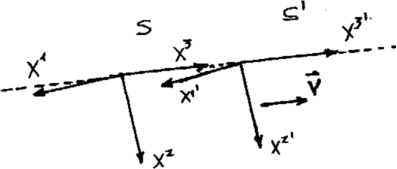
\includegraphics[width=0.4\textwidth]{images/fig_ft1_transfvec.pdf}	 
	\end{center}
	\caption{}
\end{figure} 

Se verifica entonces la transformación de Lorentz
\begin{align*}
	x^{1'} &= x^1  \\
	x^{2'} &= x^2  \\
	x^{3'} &= \gamma \: [ x^3 - \beta x^0]  \\
	x^{0'} &= \gamma \: [ x^0 - \beta x^3] 
\end{align*}
donde son 
\[
	\gamma = \frac{1}{(1 - v^2/c^2)^{1/2}} \qquad \qquad x^0 = ct 
\]

A la transformación [1] se le puede dar forma de rotación en funciones hiperbólicas como sigue
\[
	x^{0'} = x^0 \cosh( \eta ) - x^3 \sinh( \eta )
\]
\[
	x^{3'} = -x^0 \sinh( \eta ) + x^3 \cosh( \eta )
\]
donde seguimos viendo que las leyes son lineales en las coordenadas (el espacio es isótropo)
\notamargen{Debiéramos dar ideas de estas cosas importantes de relatividad especial}
\[
	\begin{pmatrix}
	 x^{0'} \\
	 x^{3'} \\
	\end{pmatrix}
	=
	\begin{pmatrix}
	\cosh( \eta ) & \sinh( \eta ) \\
	-\sinh( \eta ) & \cosh( \eta ) \\
	\end{pmatrix}
	\begin{pmatrix}
	 x^{0} \\
	 x^{3} \\
	\end{pmatrix}
\]
y no es otra cosa  que una rotación en eje $\hat{0}, \hat{3}$ con el ángulo $\eta = atanh( \beta )$. Notemos
que se verifica la invariancia del módulo de la transformación
\[
	(x^{0'})^2 -  ( (x^{1'})^2  + (x^{2'})^2 + (x^{3'})^2 ) =
		(x^{0})^2 -  ( (x^{1})^2  + (x^{2})^2 + (x^{3})^2 ) 
\]
o en una notación más feliz
\[
	(ct')^2 - ( x'^2 + y'^2 + z'^2 ) = (ct)^2 - ( x^2 + y^2 + z^2 )
\]
	
Este espacio 4D es el de Minkowski y no es euclídeo.
\[
	\begin{pmatrix}
	 x^{0'} \\
	 x^{1'} \\
	 x^{2'} \\
	 x^{3'} \\
	\end{pmatrix}
	=
	\begin{pmatrix}
	\gamma & 0 & 0 & -\beta\gamma \\
	0 & 1 & 0 & 0 \\
	0 & 0 & 1 & 0\\
	-\beta\gamma  & 0 & 0 & \gamma \\
	\end{pmatrix}
	\begin{pmatrix}
	 x^{0} \\
	 x^{1} \\
	 x^{2} \\
	 x^{3} \\
	\end{pmatrix}
\]

La transformación inversa se obtiene tomando los reemplazos
\[
	x^{i'} \to x^i \quad ,\quad  x^i \to x^{i'} \quad ,\quad  \beta \to -\beta
\]
El elemento invariante de línea es 
\[
	ds^2 = (dx^0)^2 - (dx^1)^2 - (dx^2)^2 - (dx^3)^2 = ds^{'2}
\]
o bien 
\[
	ds^2 = g_{\alpha\beta}dx^{\alpha}dx^{\beta}
\]
que es el tensor de la métrica. Se verifica
\[
	g_{\alpha\beta} = g^{\alpha\beta} =
	\begin{pmatrix}
	 1 & 0 & 0 & 0 \\
	 0 & -1 & 0 & 0 \\
	 0 & 0 & -1 & 0 \\
	 0 & 0 & 0 & -1 \\
	\end{pmatrix}
\]

\subsubsection{Cuadrivectores en el espacio 4D}

Un cuadrivector contravariante es
\[
	A^{\mu} = ( A^0, \vb{A})
\]
mientras que el covariante es
\[
	A_{\mu} = ( A^0, -\vb{A})
\]
y vemos que las partes temporales son las mismas cambiando el signo de la espacial. Las reglas de 
transformación son
\[
	A'^{\alpha}= \dpar{x'^{\alpha}}{x^{\beta}} A^{\beta} \qquad\qquad 
		A'_{\alpha}= \dpar{x^{\beta}}{x'^{\alpha}} A_{\beta}
\]
luego el producto interno es
\[
	\widetilde{A}\cdot\widetilde{B} \equiv A_\alpha B^\alpha
\]
donde estamos usando convención de suma de Einstein, que significa que 
\[
	\widetilde{A}\cdot\widetilde{B} = A^0 B^0 -\pe{A}{B}
\]
que es invariante por ser un escalar de Lorentz,
\[
	A_\alpha B^\alpha = A'_\alpha B'^\alpha
\]

\subsubsection{Intervalos entre eventos}

Los intervalos deben ser invariantes relativistas y de Lorentz, si el intervalo es temporal se tiene 
\[
	x^0 > x^i x_i \Rightarrow \delta s^2 > 0  
\]
y los eventos pueden estar conectados causalmente
\[
	x^0 < x^i x_i \Rightarrow \delta s^2 < 0 
\]
y los eventos no pueden estar conectados causalmente. Se cumple
\[
	\delta s^2 = (x^0)^2 - [ (x^1)^2 + (x^2)^2 + (x^3)^2 ]
\]

\subsubsection{Operadores diferenciales}

Tenemos la derivada respecto a una coordenada contravariante
\[
	\partial_\alpha \equiv \dpar{}{x^\alpha} = \left( \dpar{}{x^0}, \Nabla \right)
\]
que es la derivada covariante, y también la derivada respecto de una coordenada covariante
\[
	\partial^\alpha \equiv \dpar{}{x_\alpha} = \left( \dpar{}{x^0}, - \Nabla \right)
\]
que es la derivada contravariante. Note la asimetría entre derivo respecto de arriba y es derivada abajo
y viceversa. La notación abreviada puede inducir a confusiones.

La cuadridivergencia de un cuadrivector es un invariante,
\[
	\partial_\alpha A^\alpha = \dpar{A^0}{x^0} + \Nabla\cdot\vb{A}
\]
\[
	\partial^\alpha A_\alpha = \dpar{A^0}{x^0} - \Nabla\cdot(-\vb{A})
\]
y aquí vemos $\partial_\alpha A^\alpha = \partial^\alpha A_\alpha$. Esto nos lleva al D'Alembertiano
\[
	\Box \equiv \partial_\alpha \partial^\alpha = \dpar[2]{}{x^0} - \nabla^2
\]
S es el intervalo entre los eventos 1 y 2, y es un invariante lorentziano
\[
	s^2 = c^2( t_1 - t_2 )^2 - | \vb{x}_1 - \vb{x}_2 |^2
\]
El intervalo es temporal si $s^2 >0$ en cuyo caso se tiene 
\[
	c \delta t >  | \vb{x}_1 - \vb{x}_2 |
\]
lo cual significa que existe frame inercial donde $x_1=x_2$ los eventos ocurren en el mismo sitio de manera
que pueden estar conectados causalmente; puesto que $c\delta t > 0$ y $t_2>t_1$. Por el contrario si 
$c^2 < 0$ se tiene 
\[
	c \delta t <  | \vb{x}_1 - \vb{x}_2 |
\]
y existe entonces frame inercial donde los dos eventos son en el mismo sitio $x_1=x_2$ y entonces $c\delta t 
< 0$ y $t_2 < t_1$ de manera que no pueden estar conectados causalmente.

\begin{figure}[htb]
	\begin{center}
	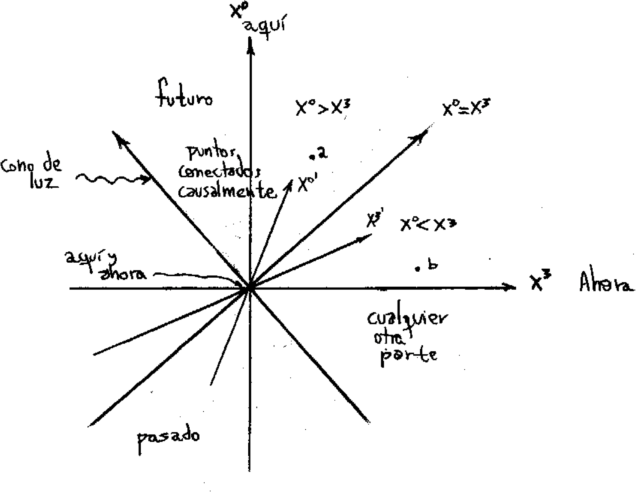
\includegraphics[width=0.6\textwidth]{images/fig_ft1_intervalos.pdf}	 
	\end{center}
	\caption{}
\end{figure} 

Según se interpreta claramente del gráfico de la figura [ampliar].
\[
	x'^0 = \gamma (x^0 - \beta x^3) \qquad x'^3 = \gamma (x^3 - \beta x^0)
\]
y si ahora es $x'^0 = 0$ entonces para un observador en $S'$ se tiene 
\[
	0 = \gamma (x^0 - \beta x^3) 
\]
o bien $x^0 = \beta x^3$ y aquí es $x'^3 = 0$ de modo que 
\[
	\frac{x^3}{\beta} = x^0
\]
y entonces $a$ de la figura puede ser causado por un suceso en el origen pero $b$ no tiene 
conexión causal con el origen.

\subsection{Transcurso del tiempo en un sistema con V grande}

Sea $v/c$ no despreciable 
\[
	c \Delta t' = \gamma ( c\Delta t - \beta \Delta z) \qquad \qquad \gamma >1
\]
\[
	\Delta t' = \gamma \Delta t \left( 1 - \beta \frac{\Delta z}{c\Delta t} \right)
\]
pero si en $S'$ la partícula está en reposo es $v = dz/dt $ de manera que 
\begin{figure}[htb]
	\begin{center}
	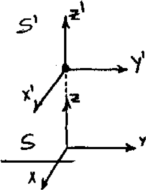
\includegraphics[width=0.3\textwidth]{images/fig_ft1_vgrande.pdf}	 
	\end{center}
	\caption{}
\end{figure} 
\[
	\Delta t' = \gamma \Delta t ( 1 - \beta^2)
\]
\[
	\Delta t' = \Delta t ( 1 - \beta^2)^{1/2}
\]
de modo que $ \Delta t' < \Delta t$, en $S'$ el tiempo transcurre más lentamente.

\subsubsection{Número de onda y conteo}

Un proceso de conteo (discreto) es invariante lorentziano
\[
	x'^3 = \gamma ( x^3 - \beta x^0 )
\]
siendo \vb{v} entre sistemas $SS'$.
El número de crestas es 
\[
	\#_s = \frac{ z_1 - z }{ \lambda } = \frac{ k }{ 2\pi }( z_1 - z ) = \frac{ k }{ 2\pi }( ct - z ) = 
	\frac{ 1 }{ 2\pi }( \omega t - kz )
\]
\[
	\#_s' = \frac{ 1 }{ 2\pi }( \omega' t' - k'z' )
\]
y se puede generalizar
\[
	\pe{k'}{x'} - \omega' t' = \pe{k}{x} - \omega t
\]
\[
	-\left( \pe{k'}{x'} - \frac{\omega' x'^0 }{c} \right) = -\left( \pe{k}{x} - \frac{\omega x^0 }{c}  
\right)
\]
es un invariante lorentziano como
\[
	k_\alpha x^\alpha = k^\alpha x_\alpha
\]
donde el cuadrivector de onda se define
\[
	k^\alpha = \left( \frac{\omega}{c}, \vb{k}\right).
\]

% =================================================================================================
\section{Forma covariante del electromagnetismo}
% =================================================================================================

Partimos de la ecuación de continuidad para la carga,
\[
	\dpar{\rho}{t} + \divem{J} = 0
\]
la cual con la definición del cuadrivector corriente
\[
	J^\mu = ( c\rho , \vb{J} )
\]
se puede escribir como 
\[
	\partial_\mu J^\mu = \dpar{c\rho}{ct} + \divem{J} = 0 .
\]

La formulación covariante empleaba el gauge de Lorentz (así las ecuaciones son validas en cualquier sistema
inercial), el gauge de Lorentz era
\[
	\frac{1}{c} \dpar{\phi}{t} + \divem{A} = 0
\]
siendo el cuadripotencial
\[
	A^\mu = ( \phi , \vb{A} ) 
\]
y entonces 
\[
	\partial_\mu A^\mu = \dpar{\phi}{ct} + \divem{A} = \frac{1}{c} \dpar{\phi}{t} + \divem{A} = 0 .
\]

Se podía ver que resultan ecuaciones de onda inhomogéneas para los potenciales
\[
	\Nabla^2 \vb{A} - \frac{1}{c^2} \dpar[2]{\vb{A}}{t} = -\frac{4\pi}{c} \vb{J}
\]
que viene a ser 
\[
	\partial_\mu\partial^\mu = \Box \vb{A} = \frac{4\pi}{c} \vb{J}
\]
y para el potencial $\phi$
\[
	\Nabla^2 \phi - \frac{1}{c^2} \dpar[2]{\phi}{t} = - 4\pi \phi
\]
que desemboca en 
\[
	\partial_\mu\partial^\mu = \Box \phi = \frac{4\pi}{c} ( c\rho )
\]

Al aplicar el D'Alembertiano a un cuadrivector obtenemos otro cuadrivector 
\[
	\Box A^\mu = \frac{4\pi}{c} J^\mu.
\]

Los campos \vb{E}, \vb{B} forman parte de un tensor de segundo rango antisimétrico llamado tensor
de intesidad de campo 
\[
	F^{\alpha\beta} = \partial^\alpha A^\beta - \partial^\beta A^\alpha
\]
que matricialmente se puede ver como 
\[
	F^{\alpha\beta} =
	\begin{pmatrix}
	 0 & -E_x & -E_y & -E_z \\
	 E_x & 0 & -B_z & B_y \\
	 E_y & B_z & 0 & -B_x \\
	 E_z & -B_y & B_x & 0 \\
	\end{pmatrix}
\]
También se suele definir un tensor de intensidad de campo dual
\[
	\mathcal{F}^{\alpha\beta} =  \frac{1}{2} \varepsilon^{\alpha\beta\gamma\delta} F_{\gamma\delta}
\]
que no es otra cosa que 
\[
	\mathcal{F}^{\alpha\beta}=
	\begin{pmatrix}
	 0 & -B_x & -B_y & -B_z \\
	 B_x & 0 & E_z & -E_y \\
	 B_y & -E_z & 0 & E_x \\
	 B_z & E_y & -E_x & 0 \\
	\end{pmatrix}
\]
y donde $\varepsilon^{\alpha\beta\gamma\delta}$ es el tensor de Levi-Civita de cuatro dimensiones, que es nulo
cuando se repite un índice.
Entonces las ecuaciones de Maxwell en forma covariante explícita resultan 
\[
	\partial_\alpha \mathcal{F}^{\alpha\beta} =  0 \qquad \qquad 
	\partial_\alpha F^{\alpha\beta} =  \frac{4 \pi}{c} J^\alpha.
\]

\subsection{Transformación de los campos}

L transformación de Lorentz era 
\begin{align*}
	ct' &= \gamma \: [ ct - \pe{\beta}{x} ] \\
	\mathbf{x'}_\parallel &= \gamma \: [ \mathbf{x}_\parallel - {\beta}ct ] \\
	\mathbf{x'}_\perp &= \mathbf{x}_\perp
\end{align*}
con $\vb{\beta} = \vb{v}/c$ y donde la transformación de los campos \vb{E}, \vb{B}

\begin{figure}[htb]
	\begin{center}
	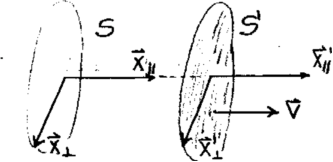
\includegraphics[width=0.4\textwidth]{images/fig_ft1_transfCampo1.pdf}	 
	\end{center}
	\caption{}
\end{figure} 

\[
	\vb{E}' = \vb{E}_\parallel + \gamma \: ( \vb{E}_\perp  + \pv{\beta}{B} )
\]
\[
	\vb{B}' = \vb{B}_\parallel + \gamma \: ( \vb{B}_\perp  - \pv{\beta}{E} )
\]
que se pueden poner como 
\[
	\vb{E}' = - \frac{ \gamma^2 }{ \gamma + 1 }\vb{\beta} (\pe{\beta}{E}) +
		\gamma \: ( \vb{E}  + \pv{\beta}{B} )
\]
\[
	\vb{B}' = - \frac{ \gamma^2 }{ \gamma + 1 }\vb{\beta} (\pe{\beta}{B}) + 
		\gamma \: ( \vb{B}  - \pv{\beta}{E} )
\]
y recordemos que la transformación de Galileo era
\[
	\vb{E}' = \vb{E} + \frac{1}{c} \pv{V}{B} \qquad \qquad 
	\vb{B}' = \vb{B} - \frac{1}{c} \pv{V}{E}
\]
siendo el segundo término el que da origen a las corrientes de Foucault al mover un conductor en el seno
de un campo \vb{B}.

\begin{figure}[htb]
	\begin{center}
	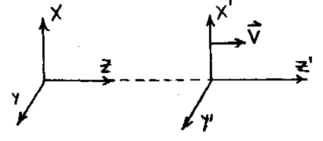
\includegraphics[width=0.4\textwidth]{images/fig_ft1_transfCampo2.pdf}	 
	\end{center}
	\caption{}
\end{figure} 

Según la figura superior la transformación de los campos satisface 
\begin{align*}
	E'_x = \gamma ( E_x - \beta B_y ) \qquad B'_x = \gamma ( B_x + \beta E_y ) \\
	E'_y = \gamma ( E_y + \beta B_x ) \qquad B'_y = \gamma ( B_y - \beta E_x ) \\
	E'_z = E_z \qquad B'_z = B_z 
\end{align*}

Las contracciones del producto escalar entre el tensor de intensidad son invariantes. Así, por ejemplo,
\begin{align*}
	F^{\alpha\beta}F_{\alpha\beta} &= 2( B^2 - E^2 ) \\
	\mathcal{F}^{\alpha\beta}\mathcal{F}_{\alpha\beta} &= 2( E^2 - B^2 ) \\
	\mathcal{F}^{\alpha\beta}F_{\alpha\beta} &= -4 \: \pe{B}{E}
\end{align*}

Sea 
\[
	\mathcal{F}^{\alpha\beta}F_{\alpha\beta} = -4 \: \pe{B}{E} = 0,
\]
entonces $\vb{E} \perp \vb{B}$ o alguno de los campos es nulo en todo sistema inercial. Para una carga 
que se mueve con velocidad \vb{v} se tiene $\vb{B}=0$ en un sistema en el que $q$ está en reposo de manera
que 
\[
	\pe{B}{E} = \pe{B'}{E'} = 0
\]
siempre y entonces $\vb{E'} \perp \vb{B'}$ para cualquier sistema inercial S'.

Un sistema electromagnético dependiente del tiempo intercambiará \vb{p} con el campo entonces no vale el
principio de acción y reacción ,
\[
	\dtot{\vb{P}_M}{t} + \dtot{\vb{P}_c}{t} = \int_{S(v)} \overline{T}\cdot d\vb{S}
\]
mientras que 
\[
	\dtot{\vb{P}_c}{t} = \dtot{}{t} \left( \frac{1}{4\pi c} \int \pv{E}{B} dV \right)
\]

\subsection{Covarianza con medios materiales}

En presencia de medios materiales puede definirse
\[
	G^{\alpha\beta} =
	\begin{pmatrix}
	 0 & -D_x & -D_y & -D_z \\
	 D_x & 0 & -H_z & H_y \\
	 D_y & H_z & 0 & -H_x \\
	 D_z & -H_y & H_x & 0 \\
	\end{pmatrix}
\]
y 
\[
	F^{\alpha\beta} \to G^{\alpha\beta}, \quad E_i \to D_i, \quad B_i \to H_i
\]
si las relaciones constitutivas son 
\[
	\vb{D} = \vb{E} + 4\pi\vb{P} \qquad\qquad \vb{H} = \vb{B} - 4\pi\vb{M}
\]
desde 
\[
	G^{\alpha\beta} = F^{\alpha\beta} + R^{\alpha\beta}
\]
y con 
\[
	\partial_\alpha G^{\alpha\beta} = \frac{4\pi}{c} J^\beta
\]
donde la información de $P_i$ y $M_i$ está en el tensor $R^{\alpha\beta}$.
Recordemos que los campos transforman según 
\[
	\vb{P}' = \vb{P}_\parallel + \gamma \: ( \vb{P}_\perp  - \pv{\beta}{M} )
\]
\[
	\vb{M}' = \vb{M}_\parallel + \gamma \: ( \vb{M}_\perp  + \pv{\beta}{P} )
\]

Entonces de un sistema inercial a otro una \vb{P} da origen a una \vb{M} y viceversa.

% =================================================================================================
\section{Principio de Hamilton y relatividad}
% =================================================================================================

% =================================================================================================
\section{Especie de tiro oblicuo}
% =================================================================================================

\begin{figure}[htb]
	\begin{center}
	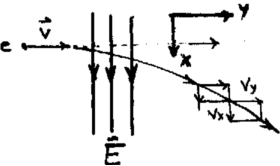
\includegraphics[width=0.4\textwidth]{images/fig_ft1_tirooblicuo.pdf}	 
	\end{center}
	\caption{}
\end{figure} 

% =================================================================================================
\section{cuadrivelocidad}
% =================================================================================================


\begin{figure}[htb]
	\begin{center}
	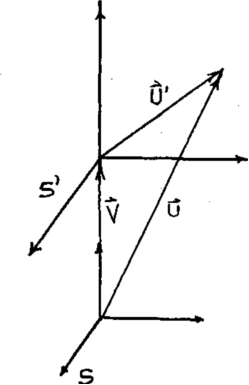
\includegraphics[width=0.4\textwidth]{images/fig_ft1_4vel.pdf}	 
	\end{center}
	\caption{}
\end{figure} 

% \bibliographystyle{CBFT-apa-good}	% (uses file "apa-good.bst")
% \bibliography{CBFT.Referencias} % La base de datos bibliográfica

\end{document}
